\section{Greedy Index Construction}
\label{preprocessing}

This section describes the greedy index construction algorithm. For a vertex, all shortest paths from a landmark can be indexed as the label of it. We study the problem of deciding which shortest path to be indexed can lead to better online query accuracy for average cases. 

\begin{figure*}[ht]
    \centering
    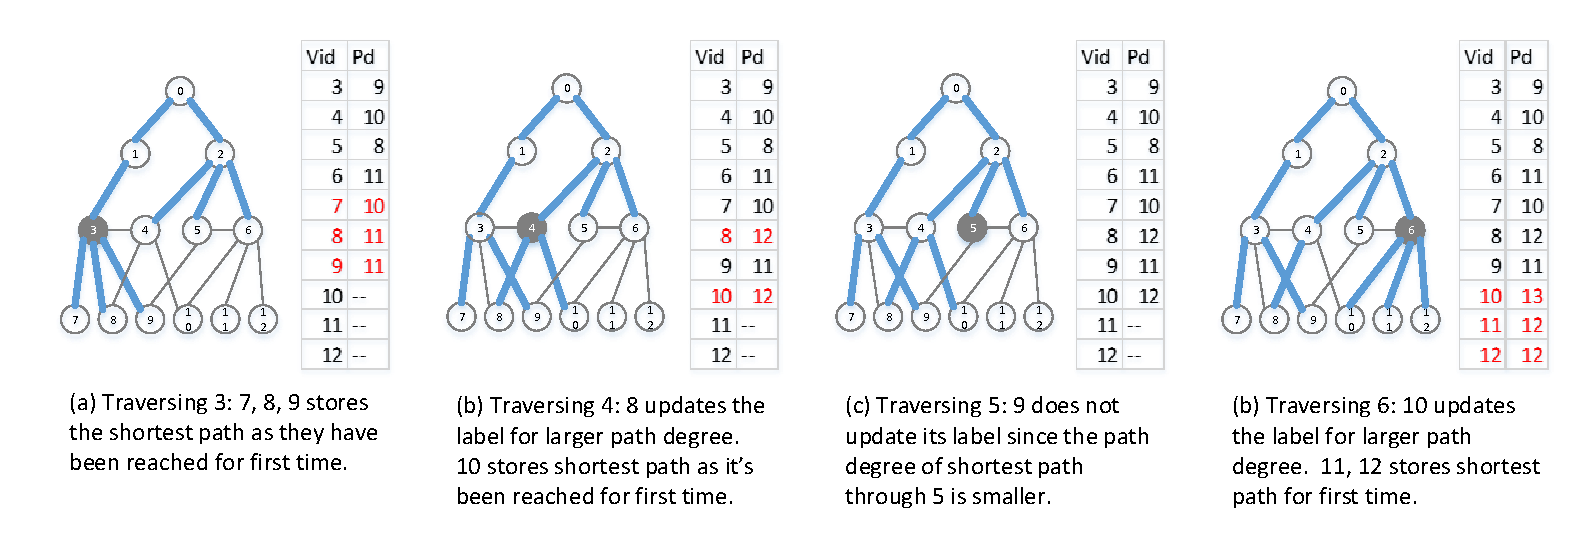
\includegraphics[width=\linewidth]{./figures/new_illustrate/bfs_illustrate.pdf}
    \caption{Heuristic index construction pick shortest path with highest path degree during breadth first search}
    \label{fig:bfs_illustrate}
\end{figure*}

As the core of decentralized search is to iteratively find neighbor vertices that has shortest LCA distance to the target. From the point of view of a vertex $u$, for landmark $l$, if the indexed shortest path $p_i$ intersects with more indexed shortest paths of other vertices, then for queries that have $u$ as target vertex, the higher the possibility that other vertices have a LCA with $u$ that is further from $l$ on shortest path tree $SPT_l$. With this intuition, we design our heuristic greedy index construction algorithm to index the shortest path with highest "centrality", i.e. intersects with most other shortest paths to increase accuracy for average cases. To represent the "centrality" of a shortest path, we use the sum of vertex centrality along the path. Although betweenness centrality fits our needs very well, the computation cost is high~\cite{Riondato:2014:FAB:2556195.2556224}. So we use degree as an alternative and refer the sum of degree of vertices along a path as path degree, denoted by $Pd$.

Index construction procedure can be easily modified to index the shortest path with highest path degree. Note that path degree of shortest path follows optimal substructure, i.e. if a shortest path $(u, .., w, ..., v)$ has the highest path degree among all the shortest paths from $u$ to $v$, then the path degree of $(u, ..., w)$ is also the highest among all the shortest paths from $u$ to $w$. To modify the index construction, during BFS, suppose the search is visiting vertex $u$ and reach its neighbor $v$ with non empty $L(v)$. A label update is performed if $|L(v)| > |L(u)|$ and $Pd(u) + \rho(v) > Pd(v)$, where $\rho(v)$ denote the degree of vertex $v$. The detailed algorithm of greedy index construction is depicted in~\ref{alg:dec}. 

Fig.~\ref{fig:bfs_illustrate} shows an example of how to greedily select shortest path with the highest path degree during breadth first search. When traversing vertex $4$, even though vertex $8$ has already been indexed with a shortest path $(0, 1, 3, 8)$ into its label, due to that $(0, 2, 4, 8)$ has a higher path degree, the label of vertex $8$ is updated. The same thing happens to vertex $10$ while traversing vertex $6$. 

\begin{algorithm}[h]
    \caption{Greedy index construction on landmark $l$}
		\label{alg:ind}
    \begin{algorithmic}
				\Function{Index construction}{$l$}
						\State For each $v$ in $G$: $L(v) \gets \emptyset$
						\State For each $v$ in $G$: $Pd(v) \gets 0$
						\State $Q \gets \emptyset$
						\State $L(l) = l$
						\State $Pd(l) = \rho(l)$ \
						\Comment {$\rho$ denotes degree}
						\State $Q.push(l)$
						\While{$Q \neq \emptyset$}
								\State $u = Q.pop()$
								\For{each $v_i$ adjecent to $u$}
										\If{$L(v_i) \neq \emptyset$}
												\State $L(v_i) = L(u)$
												\State append $v_i$ to $L(v_i)$
												\State $Pd(v_i) = Pd(u) + \rho(v_i)$
												\State $Q.push(v_i)$
										\ElsIf{$|L(v_i)| > |L(u)|$ {\bf and} $Pd(v_i) < Pd(u) + \rho(v_i)$}
												\State $L(v_i) = L(u)$
												\State append $v_i$ to $L(v_i)$
												\State $Pd(v_i) = Pd(u) + \rho(v_i)$
										\EndIf
								\EndFor
						\EndWhile
						\State \Return $L$
        \EndFunction
    \end{algorithmic}
\end{algorithm}

Note that if the landmark set is relatively large, then following the highest path degree heuristic may lead to redundant labels, i.e. similar indexed shortest path tree for multiple landmarks, which can compromise the accuracy of online search. A simple way to solve this problem is to prioritize shortest paths which overlaps fewer vertices with shortest paths that have already been indexed.